\documentclass[11pt]{article}
\usepackage[a4paper, left=1in, right=1in, top=1in, bottom=1in]{geometry}
\newcommand*{\authorfont}{\fontfamily{phv}\selectfont}
\usepackage[english, greek, main=english]{babel}
\usepackage[]{mathptmx}
\usepackage[LGR,T1]{fontenc}
\usepackage[utf8]{inputenc}
\usepackage[page,toc,titletoc,title]{appendix}  % appendix, table of contents
\usepackage{enumitem}  % package for adjusting itemize sep
\usepackage{amssymb}  % extra math fonts, like \mathbb, \mathcal
\usepackage{amsmath}
\usepackage{amsthm}
\theoremstyle{definition}
\newtheorem{definition}{Definition}
\newtheorem{example}[definition]{Example}  % example numbering depends on definition
\usepackage{abstract}
\renewcommand{\abstractname}{}    % clear the title
\renewcommand{\absnamepos}{empty} % originally center
\usepackage{tikz}
\usepackage{pgfplots}
\usepackage{xcolor}
\pgfplotsset{compat=1.16}
\usepackage{tcolorbox}
\usepackage{listings}
\usepackage{subcaption}
\usepackage{booktabs}
\usepackage{varwidth}
\usepackage[export]{adjustbox}
\usetikzlibrary{arrows}

\renewenvironment{abstract}
 {{%
    \setlength{\leftmargin}{0mm}
    \setlength{\rightmargin}{\leftmargin}%
  }%
  \relax}
 {\endlist}

\makeatletter
\def\@maketitle{%
  \newpage
%  \null
%  \vskip 2em%
%  \begin{center}%
  \let \footnote \thanks
    {\fontsize{18}{20}\selectfont\raggedright  \setlength{\parindent}{0pt} \@title \par}%
}
%\fi
\makeatother




\setcounter{secnumdepth}{0}

\usepackage{color}
\usepackage{fancyvrb}
\newcommand{\VerbBar}{|}
\newcommand{\VERB}{\Verb[commandchars=\\\{\}]}
\DefineVerbatimEnvironment{Highlighting}{Verbatim}{commandchars=\\\{\}}
% Add ',fontsize=\small' for more characters per line
\usepackage{framed}
\definecolor{shadecolor}{RGB}{248,248,248}
\newenvironment{Shaded}{\begin{snugshade}}{\end{snugshade}}
\newcommand{\AlertTok}[1]{\textcolor[rgb]{0.94,0.16,0.16}{#1}}
\newcommand{\AnnotationTok}[1]{\textcolor[rgb]{0.56,0.35,0.01}{\textbf{\textit{#1}}}}
\newcommand{\AttributeTok}[1]{\textcolor[rgb]{0.77,0.63,0.00}{#1}}
\newcommand{\BaseNTok}[1]{\textcolor[rgb]{0.00,0.00,0.81}{#1}}
\newcommand{\BuiltInTok}[1]{#1}
\newcommand{\CharTok}[1]{\textcolor[rgb]{0.31,0.60,0.02}{#1}}
\newcommand{\CommentTok}[1]{\textcolor[rgb]{0.56,0.35,0.01}{\textit{#1}}}
\newcommand{\CommentVarTok}[1]{\textcolor[rgb]{0.56,0.35,0.01}{\textbf{\textit{#1}}}}
\newcommand{\ConstantTok}[1]{\textcolor[rgb]{0.00,0.00,0.00}{#1}}
\newcommand{\ControlFlowTok}[1]{\textcolor[rgb]{0.13,0.29,0.53}{\textbf{#1}}}
\newcommand{\DataTypeTok}[1]{\textcolor[rgb]{0.13,0.29,0.53}{#1}}
\newcommand{\DecValTok}[1]{\textcolor[rgb]{0.00,0.00,0.81}{#1}}
\newcommand{\DocumentationTok}[1]{\textcolor[rgb]{0.56,0.35,0.01}{\textbf{\textit{#1}}}}
\newcommand{\ErrorTok}[1]{\textcolor[rgb]{0.64,0.00,0.00}{\textbf{#1}}}
\newcommand{\ExtensionTok}[1]{#1}
\newcommand{\FloatTok}[1]{\textcolor[rgb]{0.00,0.00,0.81}{#1}}
\newcommand{\FunctionTok}[1]{\textcolor[rgb]{0.00,0.00,0.00}{#1}}
\newcommand{\ImportTok}[1]{#1}
\newcommand{\InformationTok}[1]{\textcolor[rgb]{0.56,0.35,0.01}{\textbf{\textit{#1}}}}
\newcommand{\KeywordTok}[1]{\textcolor[rgb]{0.13,0.29,0.53}{\textbf{#1}}}
\newcommand{\NormalTok}[1]{#1}
\newcommand{\OperatorTok}[1]{\textcolor[rgb]{0.81,0.36,0.00}{\textbf{#1}}}
\newcommand{\OtherTok}[1]{\textcolor[rgb]{0.56,0.35,0.01}{#1}}
\newcommand{\PreprocessorTok}[1]{\textcolor[rgb]{0.56,0.35,0.01}{\textit{#1}}}
\newcommand{\RegionMarkerTok}[1]{#1}
\newcommand{\SpecialCharTok}[1]{\textcolor[rgb]{0.00,0.00,0.00}{#1}}
\newcommand{\SpecialStringTok}[1]{\textcolor[rgb]{0.31,0.60,0.02}{#1}}
\newcommand{\StringTok}[1]{\textcolor[rgb]{0.31,0.60,0.02}{#1}}
\newcommand{\VariableTok}[1]{\textcolor[rgb]{0.00,0.00,0.00}{#1}}
\newcommand{\VerbatimStringTok}[1]{\textcolor[rgb]{0.31,0.60,0.02}{#1}}
\newcommand{\WarningTok}[1]{\textcolor[rgb]{0.56,0.35,0.01}{\textbf{\textit{#1}}}}

\usepackage{graphicx,grffile}
\makeatletter
\def\maxwidth{\ifdim\Gin@nat@width>\linewidth\linewidth\else\Gin@nat@width\fi}
\def\maxheight{\ifdim\Gin@nat@height>\textheight\textheight\else\Gin@nat@height\fi}
\makeatother
% Scale images if necessary, so that they will not overflow the page
% margins by default, and it is still possible to overwrite the defaults
% using explicit options in \includegraphics[width, height, ...]{}
\setkeys{Gin}{width=\maxwidth,height=\maxheight,keepaspectratio}

\usepackage{titlesec}

\titleformat*{\section}{\normalsize\bfseries}
\titleformat*{\subsection}{\normalsize\itshape}
\titleformat*{\subsubsection}{\normalsize\itshape}
\titleformat*{\paragraph}{\normalsize\itshape}
\titleformat*{\subparagraph}{\normalsize\itshape}

\usepackage{natbib}
\usepackage[strings]{underscore} % protect underscores in most circumstances

\newtheorem{hypothesis}{Hypothesis}
\usepackage{setspace}

% set default figure placement to htbp
\makeatletter
\def\fps@figure{htbp}
\makeatother

\usepackage{hyperref}

% move the hyperref stuff down here, after header-includes, to allow for - \usepackage{hyperref}

\makeatletter
\@ifpackageloaded{hyperref}{}{%
\ifxetex
  \PassOptionsToPackage{hyphens}{url}\usepackage[setpagesize=false, % page size defined by xetex
              unicode=false, % unicode breaks when used with xetex
              xetex]{hyperref}
\else
  \PassOptionsToPackage{hyphens}{url}\usepackage[draft,unicode=true]{hyperref}
\fi
}

\@ifpackageloaded{color}{
    \PassOptionsToPackage{usenames,dvipsnames}{color}
}{%
    \usepackage[usenames,dvipsnames]{color}
}
\makeatother
\hypersetup{breaklinks=true,
            bookmarks=true,
            pdfauthor={Steven V. Miller (Clemson University)},
             pdfkeywords = {pandoc, r markdown, knitr},  
            pdftitle={A Pandoc Markdown Article Starter and Template},
            colorlinks=true,
            citecolor=blue,
            urlcolor=blue,
            linkcolor=magenta,
            pdfborder={0 0 0}}
\urlstyle{same}  % don't use monospace font for urls

% Add an option for endnotes. -----


% add tightlist ----------
\providecommand{\tightlist}{%
\setlength{\itemsep}{0pt}\setlength{\parskip}{0pt}}

% add some other packages ----------

% \usepackage{multicol}
% This should regulate where figures float
% See: https://tex.stackexchange.com/questions/2275/keeping-tables-figures-close-to-where-they-are-mentioned
\usepackage[section]{placeins}


% Title and author

\title{Hands-On Data Analysis for ININ Using R}

\author{\Large Prof. Dr. Cornelia Storz, M.Sc. Fei (Michael) Wang\vspace{0.05in} \newline\normalsize\emph{Management and Microeconomics, Goethe-Universität Frankfurt}  }

\date{}

% colback=white,
% colframe=white!50!black, 
% title = {Sample space: countable or uncountable?}, 
% fonttitle = \large

% set tcolorbox environment
\newtcolorbox{mybox}[1]
{
  colframe = white!50!black,
  colback  = white,
  fonttitle = \large, 
  title    = {#1}
}

\xdefinecolor{gray}{rgb}{0.4,0.4,0.4}
\xdefinecolor{blue}{RGB}{58,95,205}% R's royalblue3; #3A5FCD

\lstset{% setup listings
	language=R,% set programming language
	basicstyle=\ttfamily\small,% basic font style
	keywordstyle=\color{blue},% keyword style
        commentstyle=\color{gray},% comment style
	numbers=left,% display line numbers on the left side
	numberstyle=\scriptsize,% use small line numbers
	numbersep=10pt,% space between line numbers and code
	tabsize=3,% sizes of tabs
  commentstyle=\itshape\color{green!50!gray},
  frame=single,% single frame around code
	showstringspaces=false,% do not replace spaces in strings by a certain character
	captionpos=b,% positioning of the caption below
        breaklines=true,% automatic line breaking
        escapeinside={(*}{*)},% escaping to LaTeX
        fancyvrb=true,% verbatim code is typset by listings
        extendedchars=false,% prohibit extended chars (chars of codes 128--255)
        literate={"}{{\texttt{"}}}1{<-}{{$\bm\leftarrow$}}1{<<-}{{$\bm\twoheadleftarrow$}}1
        {~}{{$\bm\sim$}}1{<=}{{$\bm\le$}}1{>=}{{$\bm\ge$}}1{!=}{{$\bm\neq$}}1{^}{{$^{\bm\wedge}$}}1,% item to replace, text, length of chars
        alsoletter={.<-},% becomes a letter
        alsoother={$},% becomes other
        otherkeywords={!=, ~, $, \&, \%/\%, \%*\%, \%\%, <-, <<-, /},% other keywords
        deletekeywords={c}% remove keywords
}



%----------------------------begin document--------------------------------%

\begin{document}
	
% \pagenumbering{arabic}% resets `page` counter to 1 
%
% \maketitle

{% \usefont{T1}{pnc}{m}{n}
\setlength{\parindent}{0pt}
\thispagestyle{plain}
{\fontsize{18}{20}\selectfont\raggedright 
\maketitle  % title \par  

}

{
   \vskip 13.5pt\relax \normalsize\fontsize{11}{12} 
   \authorfont Prof. Dr. Cornelia Storz, M.Sc. Fei (Michael) Wang \\
   \\ 
    \emph{\small Management and Microeconomics, Goethe-Universität Frankfurt}   
}

}



\begin{abstract}
    \hbox{\vrule height .2pt width 39.14pc}
    \vskip 8.5pt % \small 

\noindent This document was prepared for students who are taking ININ course and
planning to take the exam. It is a collection of notes and codes for the
course. The notes are based on the tutorials we had in the course. I am trying
to make it concise and easy to understand. I hope it can help you to review
the course and prepare for the exam. \textit{We are living in a very noisy world,
therefore let's keep it simple and clear.} I setup a challenge for myself to
deliver a clear and concise review notes within 15 pages. This brings the trade-off,
which means some figures and tables are not included in the notes. Therefore,
you have to run the codes to see the results.  

\vskip 6pt 

\noindent I hope you enjoy reading it. I also hope you will have this notes with you
whenever you want to do some data analysis. If one day, you still refer to this
notes and find it still useful, I would be very happy to hear that.

 

\vskip 8.5pt \noindent \emph{Keywords}: econometrics, data analysis, regression models, 
empirical research, innovation, management  \par
\hbox{\vrule height .2pt width 39.14pc}

\end{abstract}

\vskip -8.5pt

 % removetitleabstract

\noindent  

% table of contents
\pagenumbering{roman}
\hypersetup{linkcolor=black}
\setcounter{tocdepth}{3}
\tableofcontents


\newpage
\pagenumbering{arabic}
\setcounter{page}{1}
\section{1 Introduction}

All statistical or econometric or machine learning models are based on 
the following assumptions:

\begin{itemize}
\tightlist
\item there are something we know - \textbf{data}
\item and something we don't know - \textbf{error} \(\epsilon\).
\end{itemize}

In summary, according to confucius, \textit{to know what we know and what we do not know}, 
that is called \textbf{wisdom}. Or like Plato said, \textit{I know that I know nothing}.
To help you to review the course, the notes will be organized as follows:

\begin{enumerate}
\tightlist 
  \item \textbf{Data}: using \texttt{data.table} to get familiar with the data
  \item \textbf{Simple linear regression}: how to estimate a simple linear regression model, how to interpret the results
  \item \textbf{Multiple linear regression}: how to estimate a multiple linear regression model, how to interpret the results, how to test the model
  \item \textbf{Introduction to logistic regression}: why do we need logistic regression
  \item \textbf{Data manipulation}: will not be tested in the exam, but it is very useful for your future work or research
\end{enumerate}


\section{2 Introduction to Data and \texttt{data.table}}



Broadly speaking, there are two kinds of data: \textbf{structured data} and 
\textbf{unstructured data}. 
Structured data is data that has a structure, such as a table, 
whereas unstructured data is data that does not have a structure, 
such as a text file. In this course, we focus on structured data. 
This means all the data we will use look like tables, such as the following one:


\begin{figure}
  \centering
  \includegraphics[width=0.97\textwidth]{../drawio/R-data-table-illustration.png}
\end{figure}


The basic syntax of data.table is summarized in the following illustration. 
\textbf{You will not be tested on the syntax of data.table in the exam}. However, 
you will be tested on the underlying concepts of data.table, such as the
type of variables (integer, character, factor, etc.). In the future if
you will be working as a data scientist, you can use data.table to do 
big data analysis. You will need to know the syntax of data.table for 
practical use not for the exam.


\begin{figure}
    \centering
    \includegraphics[width=0.97\textwidth]{../drawio/R-data-table-illustration2.png}
\end{figure}

Let's start from installing and loarding the packages we need for the course.

\lstset{language=R}   

\begin{lstlisting}
# install packages
install.packages("stargazer")
# install ISLR if you don't have it
# install.packages("ISLR")
install.packages("corrplot")
# sometimes you need to install other packages
# hopefully you can figure it out by yourself
\end{lstlisting}

After you install the packages, you can load them into R.

\begin{lstlisting}
# library for data analysis
library(data.table)
library(magrittr)
library(ggplot2)
library(knitr)
library(stargazer)
library(MASS)
library(ISLR)
library(corrplot)
\end{lstlisting}

Now, we can load the data into R and manipulate the data.

\begin{lstlisting}
# read the dataset
cis <- fread("https://shorturl.at/wBESZ")
# check structure of the dataset
str(cis)
# check the first 10 rows of the dataset
head(cis, 10)
# check the number of missing values in each column
cis %>%
    .[, .SD, .SDcols = is.double] %>%
    # check the number of missing values in each column
    sapply(function(x) sum(is.na(x))) %>%
    # sort the number of missing values in each column
    sort(decreasing = TRUE) %>%
    # convert to data.table and keep rownames as a column
    as.data.table(keep.rownames = TRUE) %>%
    # set variable names
    setnames(c("variables", "Numbe of NAs")) %>%
    # check the first 10 
    head(10) %>%
    kable("pipe)
\end{lstlisting}


\subsection{2.1 Data Visualization}

It is important to visualize the data before you start to do the analysis.
To choose the right figure, you need to know the type of variables. Here is
the summary:

\begin{itemize}
\tightlist
\item \textbf{Categorical variables}: bar chart, pie chart, etc.
\item \textbf{Continuous variables}: histogram, boxplot, etc.
\item \textbf{Categorical vs. continuous variables}: boxplot or violin or histogram with different colors
\end{itemize}

Here is a demo of how to visualize the data. You can try to run the code
and see the results.

\begin{lstlisting}
# four figures in one page
# bar chart, histogram, box plot and box plot compared
# figure size
options(repr.plot.width = 10, repr.plot.height = 10)
par(mfrow = c(2, 2))
cis %>%
    # group by branche and .N calculates the number of frequency
    .[, .N, by = branche] %>%
    # order it in a descending way
    .[order(-N)] %>%
    # get the top 10 branche (industry)
    head(10) %>%
    # plot it
    with(pie(N, labels = branche, main = "Distribution of Industries"))

# histgorma for number of employees
cis %>%
    with(hist(bges, main = "number of employees"))
# boxplot for sales
cis %>%
    with(boxplot(um18,  main = "Boxplot of Sales in 2018"))
# boxplot for log(1+sales)
cis %>%
    with(boxplot(log(1+um18), main = "Boxplot of Log Transform "))
\end{lstlisting}

When you visualize the data, it is important to check two things for 
continuous variables:
\begin{itemize}
\tightlist
\item \textbf{shape}: whether the distribution is symmetric or skewed (ideally, we prefer symmetric distribution)
\item \textbf{outliers}: outliers are extreme values that deviate from other observations on data , they may indicate a variability in a measurement, experimental errors or a novelty.
\end{itemize}

\subsection{2.2 Log Transformation}

Log transformation is a very useful tool to deal with skewed data.
When you have a skewed data, you can try to log transform it. However, it
could be tricky. You need to know the underlying theory of log transformation.
Generally speaking, log transformation is used to make the data more symmetric.
To avoid the negative values, we usually use \(\log(1+x)\) instead of \(\log(x)\).

\begin{lstlisting}
# log transform
options(repr.plot.width = 10, repr.plot.height = 10)
par(mfrow = c(2, 2))
cis %>%
    with(hist(um18, main = "Histgoram of Sales (2018)"))

cis %>%
    with(hist(log(1+um18), main = "Histogram of Log (1+sales)"))

cis %>%
    with(boxplot(um18, main = "Boxplot of Sales (2018)"))
cis %>%
    with(boxplot(log(1+um18), main = "Boxplot of Log Transform "))
\end{lstlisting}


\begin{figure}
  \centering
  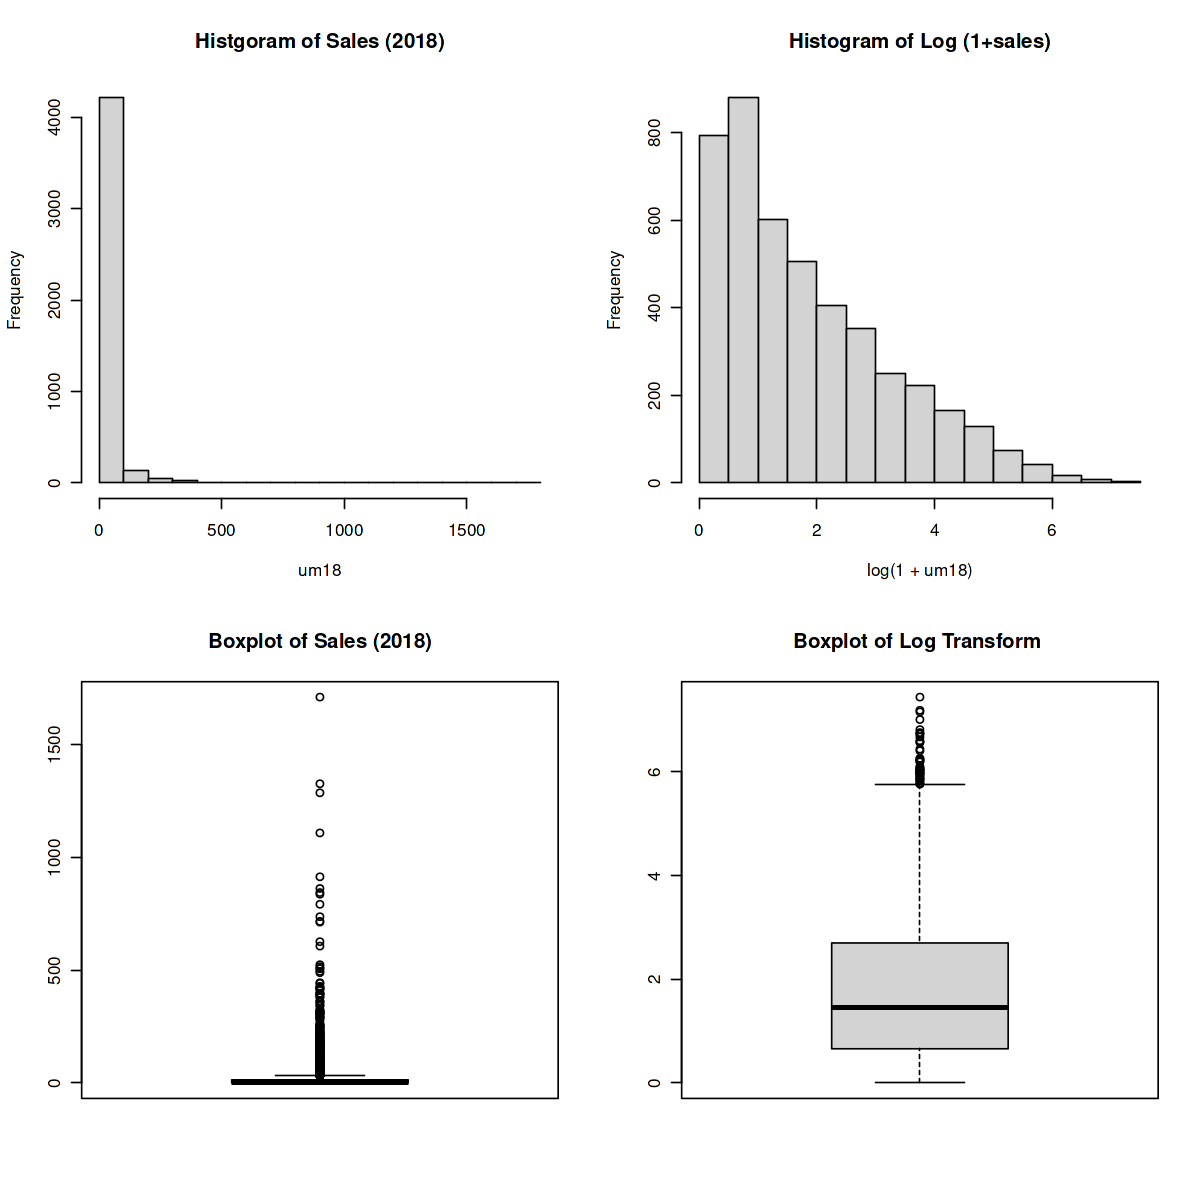
\includegraphics[width=0.9\textwidth]{./figures/vis_figure2.png}
  \caption{Log transformation of sales}
\end{figure}








\end{document}